\documentclass[a4paper]{ctexart}
\usepackage[top=3cm, bottom=2cm]{geometry}
\usepackage{graphicx}
\usepackage{subcaption}
\usepackage{amsmath}
\usepackage{amssymb}
\usepackage{xcolor}
\usepackage{url}
\usepackage{booktabs}
\usepackage{multirow}
%\usepackage{hyperref}
\usepackage[hidelinks]{hyperref} % 加载 hyperref 并隐藏链接边框

%\usepackage[utf8]{inputenc}
%\usepackage[ngerman]{babel} % 加载德语支持

% booktabs 提供 \toprule, \midrule, \bottomrule 等表格命令
% (booktabs 已在第9行加载，此处不再重复)

% 定义占位命令以避免未定义控制序列错误
%\newcommand{\placeholderspace}{}
\usepackage{fancyhdr} % 导入fancyhdr宏包
\usepackage{lipsum}   % 仅用于生成示例文本
\usepackage{float}    % 提供 H 浮动位置选项

% 设置页面样式为fancy
\pagestyle{fancy}
% 自定义页眉内容
\fancyhead[L]{} % 左侧页眉
\fancyhead[C]{\textbf{Physics-experiment Reporting Letter:\\Raman Spectroscopy}} % 中间页眉
\fancyhead[R]{} % 右侧页眉
% 自定义页脚内容
\fancyfoot[L]{} % 左侧页脚
\fancyfoot[C]{\thepage} % 中间页脚显示页码
\fancyfoot[R]{} % 右侧页脚
% 改变页眉线的粗细
\renewcommand{\headrulewidth}{1.4pt}
% 改变页脚线的粗细
\renewcommand{\footrulewidth}{0pt}

\title{拉曼光谱}
\author{实验人：学生\qquad 学号：[学号已脱敏]\qquad 指导教师：何聪丽}
\date{实验日期：2026.4.17}

\begin{document}
    
    \maketitle
    
    \begin{abstract}
        本实验以半导体激光器泵浦的 Nd$^{3+}$:YVO$_4$ 晶体经倍频产生的 532\,nm 激光作为激发光源，对四氯化碳（CCl$_4$）分子的拉曼光谱进行了测量与分析。实验中通过调节单色仪、光电倍增管以及光子计数系统等装置，成功获得了 CCl$_4$ 的拉曼散射谱，并对各特征峰的退偏度进行了测定。

        实验结果表明，CCl$_4$ 分子存在四种典型的振动模式，对应多个明显的拉曼位移峰。其中，瑞利散射线位于 532\,nm 附近，Stokes 线分布在长波长一侧，而反 Stokes 线位于短波长一侧。通过对不同谱线进行定点测量发现，各振动模式的退偏度存在显著差异，反映了分子振动对称性的不同。

        具体而言，部分谱线对应的退偏度接近零，表明其振动模式具有较高的对称性（如对称伸缩振动）；而另一部分谱线的退偏度接近 $3/4$，则表明对应振动模式对称性较低。实验结果与拉曼散射理论对分子振动对称性的预期相一致。

        \textbf{关键词：拉曼光谱 \quad 分子振动 \quad 退偏度 \quad 单光子计数}
    \end{abstract}
    
    \section{引言}

        拉曼散射是光与物质相互作用的重要现象之一。自 \text{C. V. Raman} 于 1928 年发现该效应以来，拉曼光谱已成为研究分子振动与结构的重要手段。通过分析散射光相对于入射光的频移信息，可以获得分子振动能级及其对称性特征，从而为分子结构研究提供关键依据。

        四氯化碳（CCl$_4$）是一种具有高度对称性的四面体分子，其振动模式清晰且具有典型性，因而常被选作拉曼光谱实验的标准样品。不同振动模式在拉曼光谱中对应不同的频移与退偏特性，这些特征可用于区分振动的对称性，并验证拉曼选择定则。

        本实验以 532\,nm 激光为激发光源，利用单色仪与光电倍增管组成的检测系统，对 CCl$_4$ 的拉曼散射光谱进行测量，并进一步分析各特征谱线的退偏度。通过实验数据的处理与对比，旨在加深对拉曼散射机理及分子振动对称性的理解。  

    \section{原理}

        \subsection{分子振动与拉曼散射机制}

            由 $N$ 个原子组成的分子具有 $3N$ 个自由度。对于非线性分子，其自由度可分解为 3 个平动自由度、3 个转动自由度以及 $3N-6$ 个振动自由度。各振动模式可用简正坐标 $(q_1,\dots,q_{3N-6})$ 描述，对应振动频率 $\omega_1,\dots,\omega_{3N-6}$（可能存在简并）。

            当频率为 $\omega_0$ 的入射电磁波
            \begin{equation}
                \mathbf{E} = \mathbf{E}_0 \cos \omega_0 t
            \end{equation}
            作用于分子时，会诱导产生电偶极矩
            \begin{equation}
                \mathbf{P} = \boldsymbol{\alpha}\mathbf{E}
            \end{equation}
            其中极化率张量 $\boldsymbol{\alpha}$ 是振动坐标的函数。对其在平衡位置处作泰勒展开：
            \begin{equation}
                \alpha_{ij} = (\alpha_{ij})_0 + \sum_{k}\left(\frac{\partial \alpha_{ij}}{\partial q_k}\right)_0 q_k + \cdots
            \end{equation}

            若分子振动形式为
            \begin{equation}
                q_k = Q_k \cos(\omega_k t + \varphi_k)
            \end{equation}

            代入电偶极矩表达式 $\mathbf{P} = \boldsymbol{\alpha}\mathbf{E}$，可得
            \begin{equation}
                \mathbf{P} \sim \cos \omega_0 t + \cos(\omega_0 \pm \omega_k)t
            \end{equation}

            因此，散射光中包含三类频率分量：
            \begin{itemize}
                \item $\omega_0$：瑞利散射
                \item $\omega_0 - \omega_k$：Stokes 线
                \item $\omega_0 + \omega_k$：反 Stokes 线
            \end{itemize}

            只有当
            \begin{equation}
                \left(\frac{\partial \alpha}{\partial q_k}\right)_0 \neq 0
            \end{equation}
            时，对应振动模式才是拉曼活性的。

            由于各振动态布居数满足玻尔兹曼分布
            \begin{equation}
                N \propto \exp\left(-\frac{E}{kT}\right)
            \end{equation}
            低能级粒子数更多，因此 Stokes 线强度通常大于反 Stokes 线。

        \subsection{拉曼散射退偏度}

            设散射平面为入射光传播方向与散射方向构成的平面。定义散射光强 $I$ 的偏振分量，则退偏度可表示为
            \begin{equation}
                \rho = \frac{I_{\perp}}{I_{\parallel}}
            \end{equation}
            其中 $I_{\parallel}$ 与 $I_{\perp}$ 分别表示散射光偏振方向平行与垂直于参考方向的分量。

            对于各向同性分子，在理想条件下不同振动模式的退偏度满足：
            \begin{equation}
                \rho = 0 \quad (\text{完全对称模}), \qquad \rho = \frac{3}{4} \quad (\text{非对称模})
            \end{equation}
            因此退偏度可以作为判断分子振动对称性的判据。

        \subsection{单光子计数原理}

            光子流量 $R$ 定义为单位时间内通过的光子数，光功率满足
            \begin{equation}
                P = R h \nu
            \end{equation}

            当光强极弱时（$P \lesssim 10^{-16}\ \mathrm{W}$），单位时间内的光子数接近离散统计过程，此时可通过光电倍增管（PMT）将单个光子的入射转化为电脉冲信号，并进行计数，从而实现对微弱光信号的测量。

            \begin{figure}[h!]
                \centering
                \begin{subfigure}{0.46\textwidth}
                    \centering
                    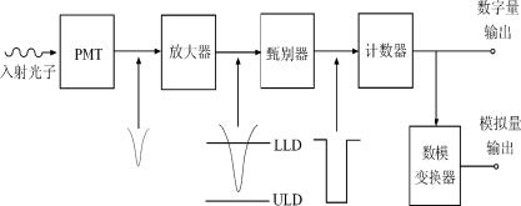
\includegraphics[width=\textwidth]{figs/4}
                    \caption{光子计数系统}
                \end{subfigure}
                \hfill
                \begin{subfigure}{0.46\textwidth}
                    \centering
                    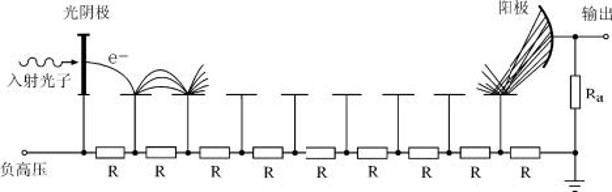
\includegraphics[width=\textwidth]{figs/5}
                    \caption{PMT 结构示意}
                \end{subfigure}
                \caption{单光子计数原理}
                \label{fig:figure3b}
            \end{figure}

        \subsection{CCl$_4$ 分子的振动模式}

            四氯化碳（CCl$_4$）为正四面体结构（$T_d$ 点群），共有
            \begin{equation}
                3N - 6 = 9
            \end{equation}
            个振动自由度。考虑对称性简并后，仅对应四种不同振动频率：
            \begin{itemize}
                \item $\nu_1$（A$_1$）：对称伸缩振动
                \item $\nu_2$（E）：弯曲振动（二重简并）
                \item $\nu_3$（F$_2$）：反对称伸缩（三重简并）
                \item $\nu_4$（F$_2$）：弯曲振动（三重简并）
            \end{itemize}

            其拉曼谱线强度一般满足
            \begin{equation}
                I_1 > I_4 > I_2 > I_3
            \end{equation}

            \begin{figure}[h!]
                \centering
                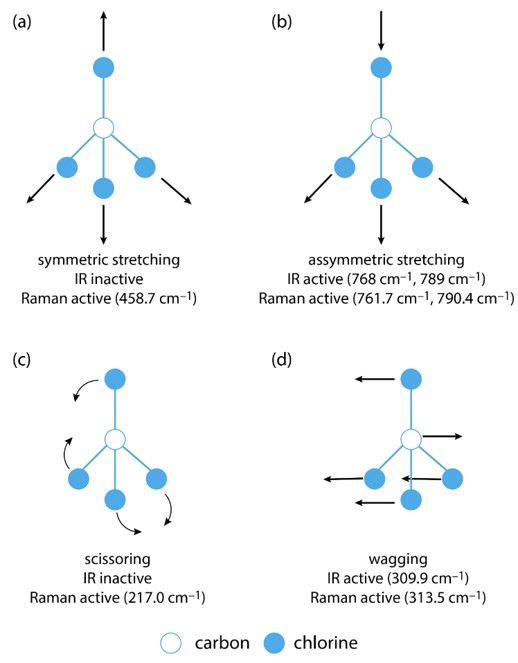
\includegraphics[width=0.5\textwidth]{figs/6}
                \caption{CCl$_4$ 分子的振动模式示意图}
                \label{fig:figure}
            \end{figure}
    
    \section{实验}

        \subsection{实验仪器}

            本实验采用半导体激光器泵浦的 Nd$^{3+}$:YVO$_4$ 激光系统作为激发光源，经倍频后输出波长为 $532\ \mathrm{nm}$ 的单色光。主要实验装置包括：

            \begin{itemize}
                \item 激光光源系统（Nd:YVO$_4$ + 倍频模块）
                \item 单色仪（用于波长扫描与分光）
                \item 光电倍增管（PMT）及单光子计数系统
                \item 起偏器与检偏器（用于偏振分析）
                \item CCl$_4$ 样品池
                \item 成像透镜与反射光学系统
            \end{itemize}

            上述装置共同构成拉曼光谱测量系统，其中单色仪用于分辨不同波长的散射光，光电倍增管用于弱光信号探测，单光子计数系统实现对微弱光信号的统计测量。

        \subsection{实验步骤}

            实验按照“系统校准—光谱测量—偏振分析—探测特性研究”的顺序进行。

            \begin{enumerate}

                \item \textbf{暗计数与阈值设定} \\
                在关闭激光光源条件下，记录系统的暗计数脉冲幅度分布。通过“阈值窗口”观察脉冲幅度曲线，选择噪声峰右侧的第一个极小值作为判别阈值，从而有效抑制噪声计数。根据该阈值设置主程序参数，为后续单光子计数测量提供可靠基准。

                \item \textbf{拉曼光谱获取与光路优化} \\
                打开激光光源，调节光路使入射激光与 CCl$_4$ 样品轴线同轴，并通过成像透镜与反射镜系统使散射光准确聚焦于单色仪狭缝中心。

                初步设置扫描范围为 $510\sim560\ \mathrm{nm}$，步长 $0.1\ \mathrm{nm}$，进行全谱扫描，获得拉曼散射谱的整体分布。

                在此基础上，采用定点测量模式（典型波长如 $546.5\ \mathrm{nm}$），通过微调光学元件位置，使探测信号强度达到最大。同时在保证信号强度的前提下逐步减小狭缝宽度，以提高光谱分辨率。进一步在局部波段（如 $555\sim557\ \mathrm{nm}$）进行精细扫描，以分辨相邻谱线结构。

                \item \textbf{退偏度测量} \\
                在光路中加入起偏器，使入射光成为线偏振光。选取典型拉曼峰（如 $545.1\ \mathrm{nm}$）进行定点测量，通过旋转检偏器，分别测量散射光在平行与垂直偏振方向上的强度极值，从而确定退偏度。

                在完成定点测量后，进一步对整个光谱进行扫描，以分析不同振动模式对应的偏振特性。

                \item \textbf{单光子计数特性分析} \\
                选取典型波长（如 $\lambda = 555.3\ \mathrm{nm}$），分别测量暗计数、拉曼峰及瑞利散射对应的脉冲幅度分布。通过比较不同情况下的脉冲幅度曲线，分析信号与噪声的区分特征，从而验证单光子计数系统的工作性能.

            \end{enumerate}

    \section{结果与分析讨论}

\subsection{暗计数脉冲噪声}

在未开启光源的条件下，通过“阈值窗口”测量得到暗计数的脉冲幅度分布曲线，如图\ref{fig:darkCountCurve}所示。由积分曲线可以确定暗计数主要来源于光电倍增管中的热电子发射，其对应脉冲幅度分布形成明显峰值。根据该曲线选取阈值为 16，以有效滤除热电子噪声。

\begin{figure}[h!]
    \centering
    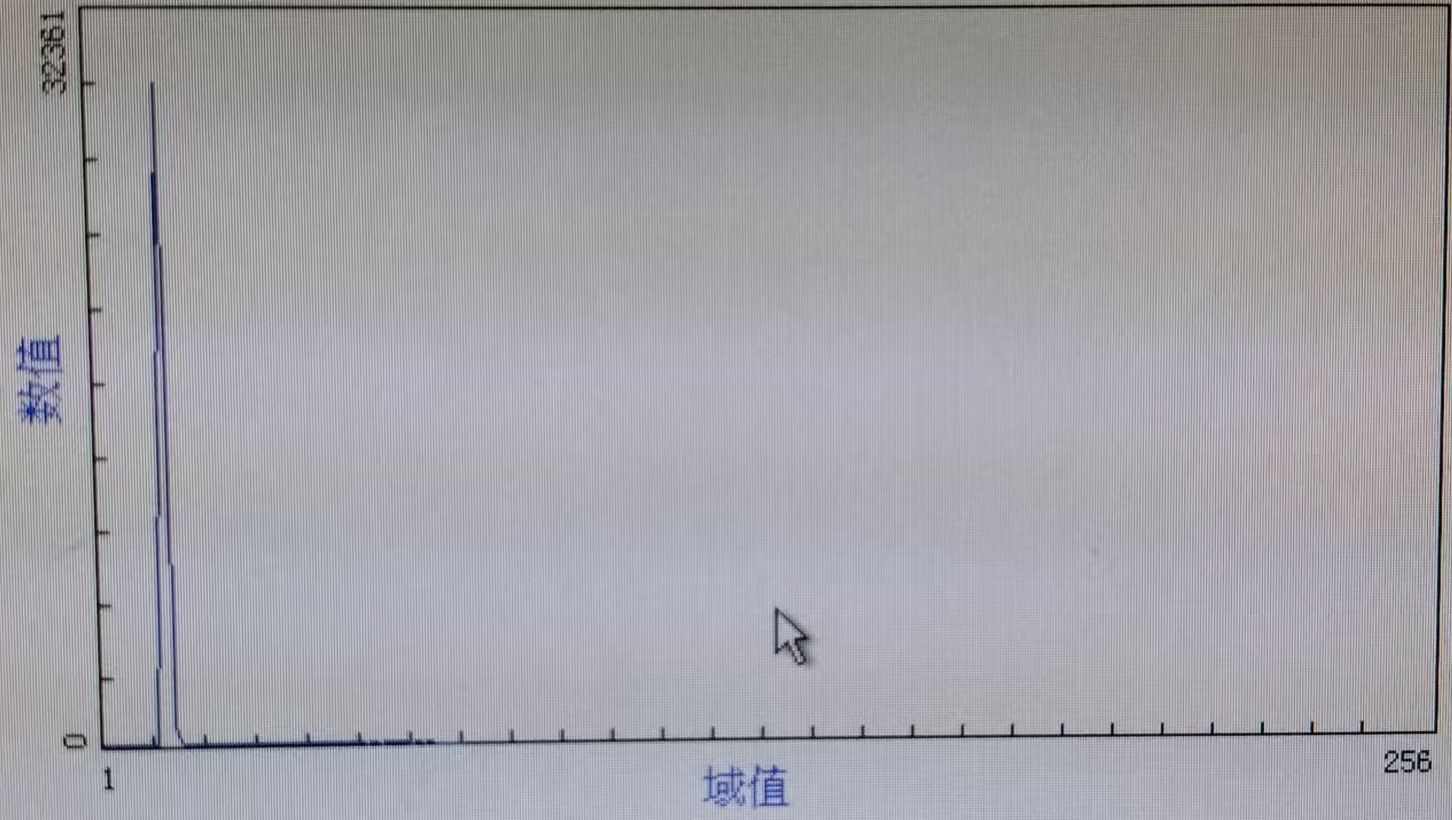
\includegraphics[width=0.8\textwidth]{figs//cut_dark}
    \caption{暗计数脉冲幅度曲线}
    \label{fig:darkCountCurve}
\end{figure}

阈值的选择需要在抑制噪声与保留有效信号之间进行权衡：阈值过低会引入大量噪声计数，而阈值过高则可能截断真实的光电子脉冲。因此选取噪声峰右侧的第一个极小值作为阈值，是一种兼顾信噪比与探测效率的合理策略。

\subsection{CCl$_4$ 的拉曼光谱}

在采用光电倍增管进行单光子计数的过程中，由于瑞利散射光强远大于拉曼散射光，系统容易出现计数饱和现象。其典型特征表现为瑞利峰顶部出现“凹陷”，这一现象来源于单光子计数系统的非线性响应，而不同于常规探测器中的饱和削顶效应。

因此，在初次获取光谱后，需要通过调节狭缝宽度控制入射光强，以避免瑞利峰过载。同时，减小狭缝宽度还能提高光谱分辨率，从而更清晰地区分相邻谱线。

在完成光路优化后，测得 CCl$_4$ 的拉曼光谱如图\ref{fig:ramanSpectrum1}与图\ref{fig:ramanSpectrum2}所示。

\begin{figure}[h!]
    \centering
    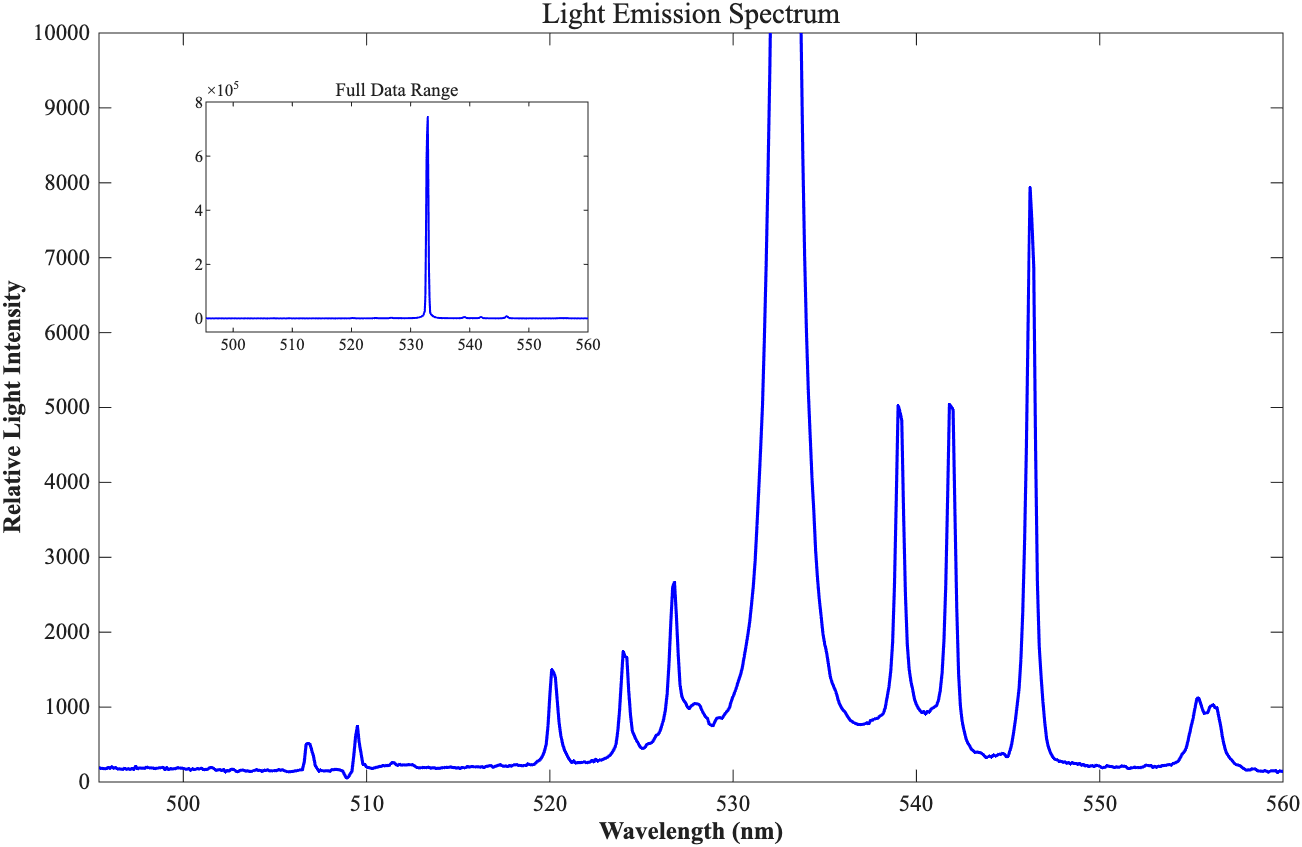
\includegraphics[width=\textwidth]{figs//raman1}
    \caption{CCl$_4$ 的拉曼光谱（波长为横坐标）}
    \label{fig:ramanSpectrum1}
\end{figure}

\begin{figure}[h!]
    \centering
    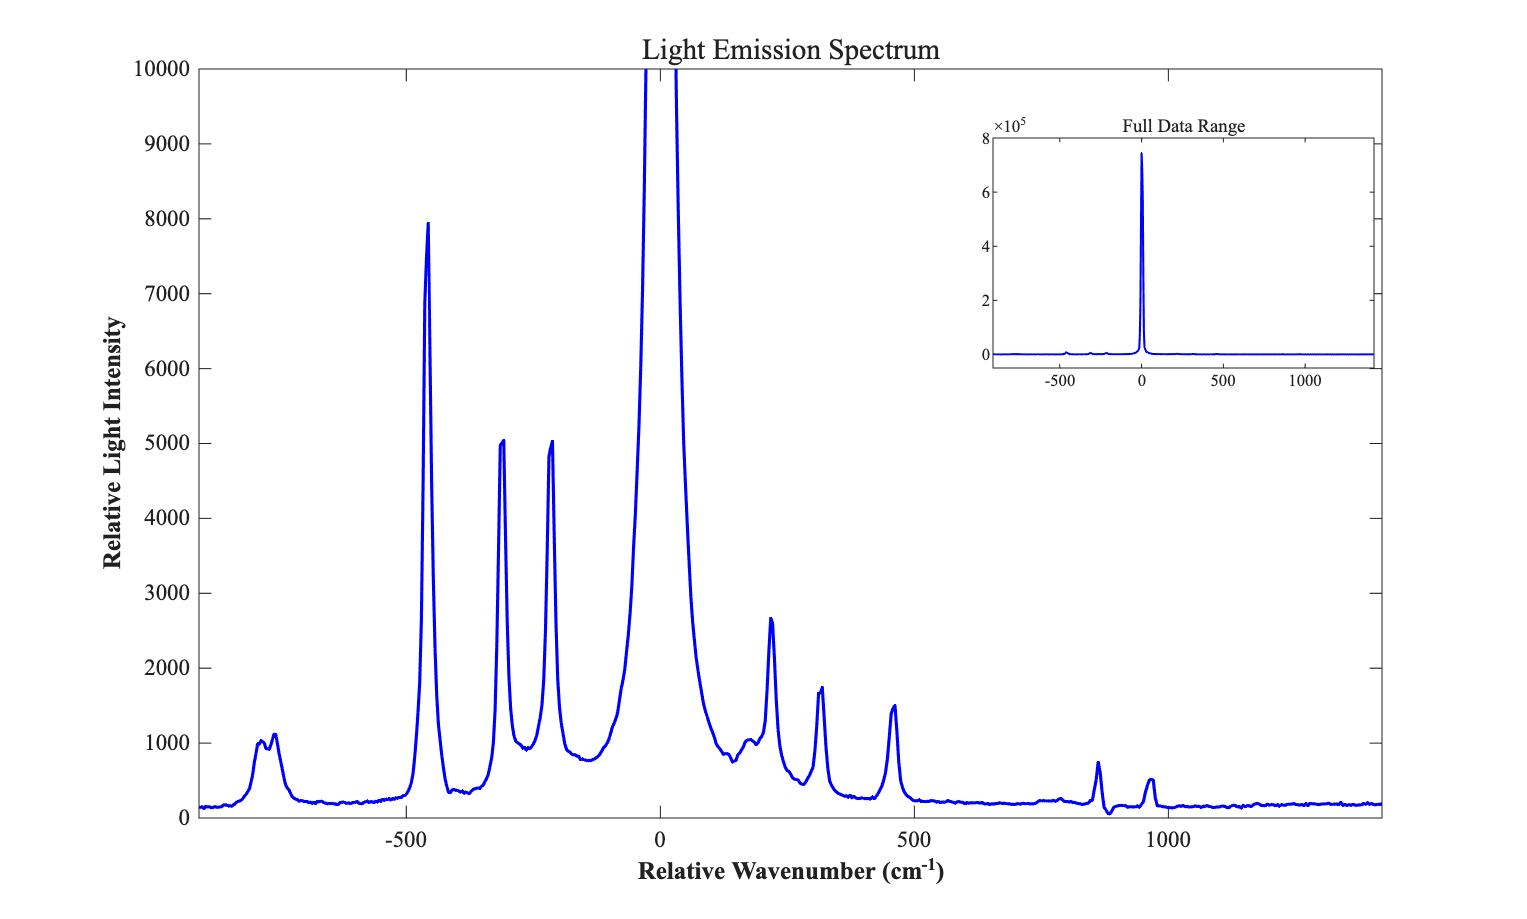
\includegraphics[width=\textwidth]{figs//raman2}
    \caption{CCl$_4$ 的拉曼光谱（波数为横坐标，基准为瑞利峰）}
    \label{fig:ramanSpectrum2}
\end{figure}

由图可见，在 532 nm 附近存在强烈的瑞利散射峰。其右侧为 Stokes 线，对应分子由低能级跃迁至高振动态；左侧为 anti-Stokes 线，对应高能级向低能级跃迁。由于热平衡下高能级粒子布居数较少，anti-Stokes 线强度明显弱于 Stokes 线，这与玻尔兹曼分布的理论预期一致。

实验中共观测到四组主要的 Stokes 拉曼峰，对应 CCl$_4$ 分子的四种基本振动模式。其中高波数区域出现双峰结构，可归因于 Fermi 共振效应，即不同振动模式之间的能级耦合导致谱线分裂。

实验测得的峰位如表\ref{tab:spectrum_1}所示，整体与理论振动频率符合良好。

\begin{table}[h]
    \centering
    \caption{拉曼光谱测量结果}
    \label{tab:spectrum_1}
    \begin{tabular}{cccccccccc}
        \toprule
        & peak 1  & peak 2 & peak 3 & peak 4 & peak 5 & peak 6 & peak 7 & peak 8 & peak 9 \\
        \midrule
        $\lambda$/nm & 520.1 & 524.0 & 526.8 & 532.9 & 539.0 & 541.8 & 546.2 & 555.4 & 556.2 \\
        $\sigma$/cm$^{-1}$ & 461.8 & 318.7 & 217.3 & 0.0 & -212.4 & -308.3 & -456.9 & -760.2 & -786.1 \\
        \bottomrule
    \end{tabular}
\end{table}

\subsection{CCl$_4$ 退偏度测量}

实验中固定入射光偏振方向，并分别测量散射光在平行与垂直偏振方向上的强度，从而计算退偏度。

需要指出的是，由于起偏器方向不可调节，入射偏振与理想几何构型之间可能存在偏差，从而引入系统误差。此外，瑞利散射具有极强强度，其尾部会对邻近拉曼峰产生背景干扰。

\begin{figure}[h!]
    \centering
    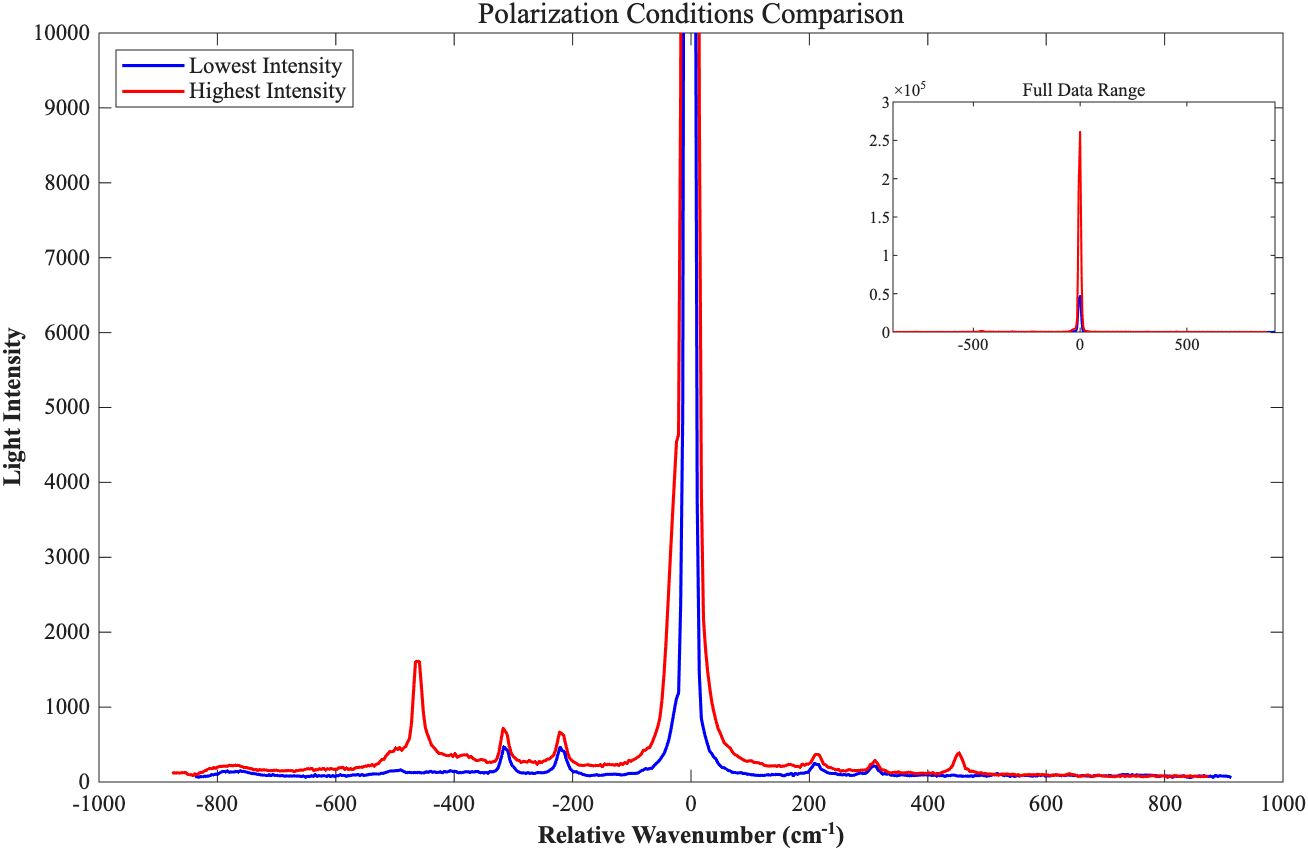
\includegraphics[width=\textwidth]{figs//raman3}
    \caption{CCl$_4$ 拉曼光谱退偏测量}
    \label{fig:polarizationDegreeMeasurement}
\end{figure}

本实验采用拉曼峰两侧平均光强作为背景估计，并对原始数据进行修正。处理后结果如表\ref{tab:spectrum_2}所示。

\begin{table}[h!]
    \centering
    \caption{退偏度测量结果}
    \label{tab:spectrum_2}
    \begin{tabular}{cccccccc}
        \toprule
        & peak 1 & peak 2 & peak 3 & peak 4 & peak 5 & peak 6 & peak 7 \\
        \midrule
        $^\perp I_\parallel$ & 消光 & 125.6 & 136.2 & \textbackslash & 147.9 & 224.3 & 151.0 \\
        $^\perp I_\perp$ & 388.9 & 289.1 & 372.0 & 261455.6 & 667.7 & 717.3 & 1614.0 \\
        退偏度 & $\approx$0 & 0.43 & 0.37 & \textbackslash & 0.22 & 0.31 & 0.09 \\
        \bottomrule
    \end{tabular}
\end{table}

\begin{figure}[h!]
    \centering
    \includegraphics[width=\textwidth]{figs//7}
    \caption{CCl$_4$ 拉曼光谱不同偏振条件下的测量}
    \label{fig:polarizationDegreeMeasurement}
\end{figure}

实验结果表明，两类振动模式具有显著不同的退偏特性：

\begin{itemize}
    \item $\rho \approx 0$ 的谱线对应完全对称振动模式（A$_1$），即各向同性的呼吸振动；
    \item $\rho \approx 3/4$ 的谱线对应非完全对称振动模式（E 或 F$_2$），表现出各向异性极化特征。
\end{itemize}

尽管部分测量值偏离理论值 $3/4$，但整体趋势与分子对称性分析一致。偏差主要来源于背景扣除方法的近似性以及瑞利散射尾部的影响。

\subsection{光子计数下脉冲幅度曲线}

\subsubsection{拉曼峰脉冲特性}

选取 $\lambda = 541.8\ \mathrm{nm}$（Stokes 峰）进行测量，得到脉冲幅度分布如图\ref{fig:ramanPeakPulse}所示。与暗计数相比，拉曼信号对应的脉冲幅度分布整体右移且峰值增强，说明信号强度显著高于噪声背景。

\begin{figure}[h!]
    \centering
    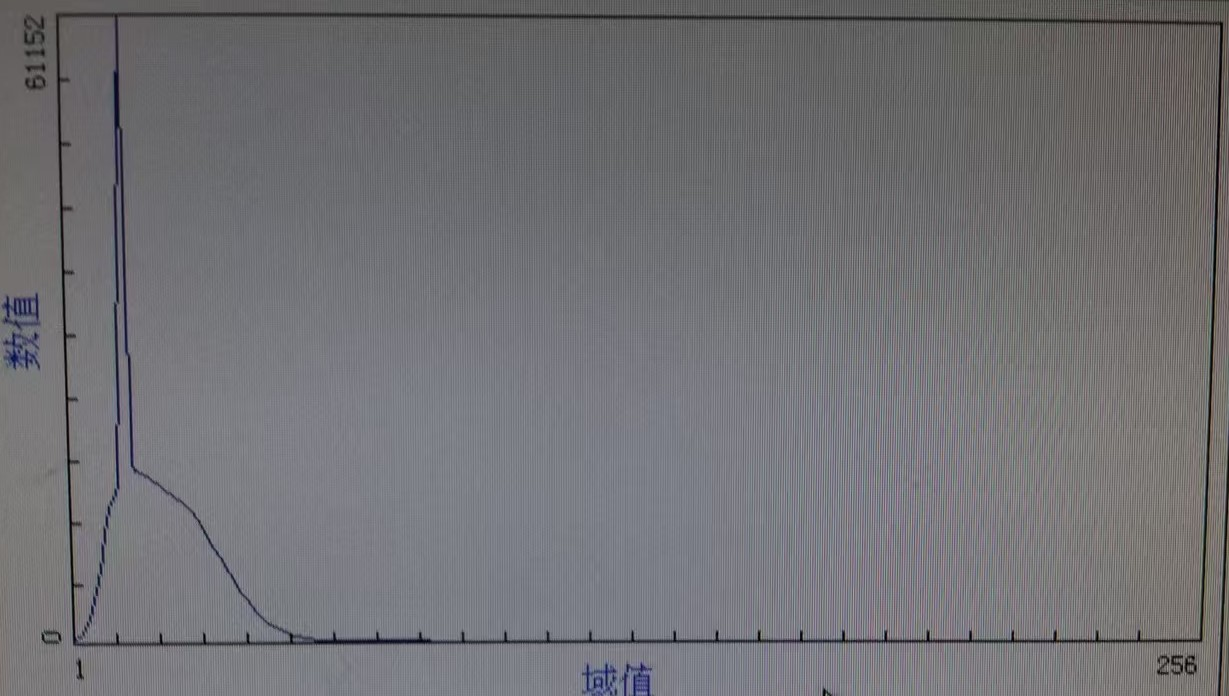
\includegraphics[width=0.8\textwidth]{figs//cut_anotherpeak}
    \caption{拉曼峰脉冲幅度分布}
    \label{fig:ramanPeakPulse}
\end{figure}

同时可以观察到脉冲分布展宽，这是由于单光子信号与电子倍增过程中的统计涨落共同作用的结果。

\subsubsection{瑞利峰脉冲特性}

选取 $\lambda = 528.0\ \mathrm{nm}$（瑞利峰），测得脉冲分布如图\ref{fig:rayleighPeakPulse}所示。此时信号强度远大于暗计数水平，噪声贡献可以忽略，阈值的选取对测量结果影响较小。

\begin{figure}[h!]
    \centering
    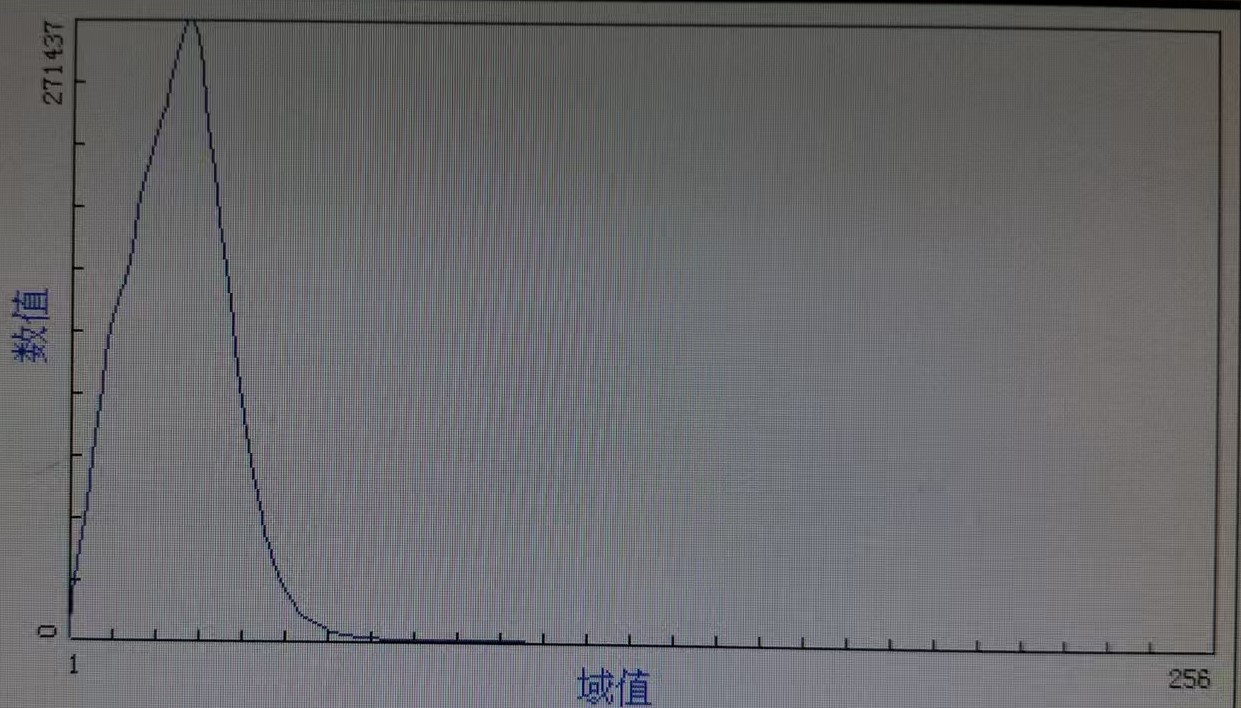
\includegraphics[width=0.8\textwidth]{figs//cut_maxpeak}
    \caption{瑞利峰脉冲幅度分布}
    \label{fig:rayleighPeakPulse}
\end{figure}

这一结果进一步表明，在强信号条件下，单光子计数系统的测量误差主要由统计涨落决定，而非电子噪声。

    \section{总结}

本实验基于单光子计数技术，对 CCl$_4$ 分子的拉曼光谱进行了系统测量，并进一步分析了其分子振动模式的对称性及对应的退偏特性。通过对光路的精细调节以及测量参数的优化，成功获得了具有良好信噪比和分辨率的拉曼光谱。

实验结果表明，CCl$_4$ 分子在本实验条件下能够清晰分辨出四种主要振动模式，其对应的拉曼峰位置与理论预期基本一致。同时，通过退偏度的测量与分析，可以将不同谱线归类为对称振动（$\rho \approx 0$）与非对称振动（$\rho \approx 3/4$）两类，从而验证了拉曼散射中极化性质与分子对称性的内在联系。

在实验过程中也暴露出若干限制因素。首先，由于瑞利散射强度远高于拉曼散射，单光子计数系统在强信号区域出现非线性响应，导致谱线中心区域的数据失真；其次，瑞利峰尾部对邻近拉曼峰的背景干扰，使退偏度的计算依赖于近似的背景扣除方法，从而引入系统误差。此外，起偏器方向不可调带来的几何偏差，也在一定程度上影响了偏振测量的准确性。

针对上述问题，可以从以下几个方面进行改进：一是通过进一步优化光学系统（如采用更窄带滤光片或提高单色仪分辨率）以抑制瑞利散射的影响；二是增加瑞利峰附近的数据采样点，从而采用更合理的函数形式进行背景拟合；三是引入可调偏振器以改善偏振测量的几何条件；四是通过延长计数时间或优化探测参数，提高弱信号测量的统计精度。

总体而言，本实验较好地实现了从拉曼光谱测量到分子对称性分析的完整实验流程，不仅验证了拉曼散射的基本理论关系，也加深了对单光子探测技术及其测量局限性的理解。
   
    \begin{thebibliography}{99}
        \bibitem{1}
        北京师范大学物理实验教学中心. 近代物理实验讲义一 (2019)
    \end{thebibliography}


\end{document}
